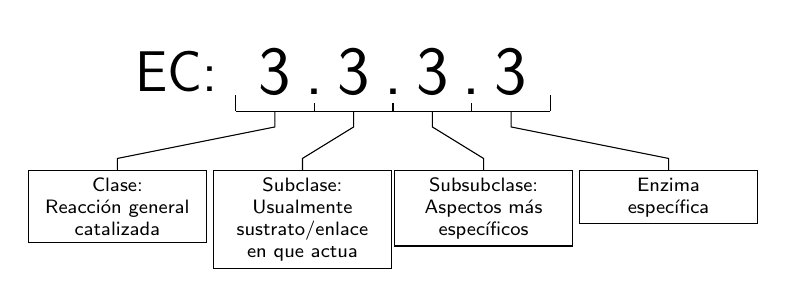
\begin{tikzpicture}
    
    \node[draw=none, node font=\huge\sffamily] at (-1.25,0) {EC:};
    \node[draw=none, node font=\Huge\sffamily] at (0,0) {3};
    \node[draw=none, node font=\Huge\sffamily] at (0.5,-0.25) {.};
    \node[draw=none, node font=\Huge\sffamily] at (1,0) {3};
    \node[draw=none, node font=\Huge\sffamily] at (1.5,-0.25) {.};
    \node[draw=none, node font=\Huge\sffamily] at (2,0) {3};
    \node[draw=none, node font=\Huge\sffamily] at (2.5,-0.25) {.};
    \node[draw=none, node font=\Huge\sffamily] at (3,0) {3};
  
    \draw (-0.5,-0.5) -- (3.5,-0.5);
    \draw (-0.5,-0.5) -- (-0.5, -0.3);
    \draw (0.5,-0.5) -- (0.5, -0.4);
    \draw (1.5,-0.5) -- (1.5, -0.4);
    \draw (2.5,-0.5) -- (2.5, -0.4);
    \draw (3.5,-0.5) -- (3.5, -0.3);

    \node[anchor=north, draw, text width=8em, align=center, node font=\scriptsize\sffamily] (clase) at (-2,-1.25) {Clase:\\Reacción general catalizada};
    \node[anchor=north, draw, text width=8em, align=center, node font=\scriptsize\sffamily] (subclase) at (0.35,-1.25) {Subclase:\\Usualmente sustrato/enlace en que actua};
    \node[anchor=north, draw, text width=8em, align=center, node font=\scriptsize\sffamily] (subsubclase) at (2.65,-1.25) {Subsubclase:\\Aspectos más específicos};
    \node[anchor=north, draw, text width=8em, align=center, node font=\scriptsize\sffamily] (enzima) at (5,-1.25) {Enzima\\específica};

    \draw (0,-0.5) --(0,-0.7) -- (-2,-1.1) -- (clase.north);
    \draw (1,-0.5) --(1,-0.7) -- (0.35,-1.1) -- (subclase.north);
    \draw (2,-0.5) --(2,-0.7) -- (2.65,-1.1) -- (subsubclase.north);
    \draw (3,-0.5) --(3,-0.7) -- (5,-1.1) -- (enzima.north);

\end{tikzpicture}